\documentclass[30px]{article}
\usepackage{fancyhdr}
\usepackage{authblk}
\usepackage{graphicx}
\usepackage{titletoc}
\font\tfont=cmr12 at 35pt
\title{{\tfont Computer Workshop Assignment No.6}}
\author{Morteza Rahimi}
\affil{Iran University of Science and Technology}
\date{Fall 4031}
\pagestyle{fancy}
\lhead{Morteza Rahimi}
\rhead{Computer Workshop Assignment No.6}
\author{Morteza Rahimi}

\begin{document}
\maketitle
\newpage
\tableofcontents
\newpage
\section{Git and Github}
\subsection{Repository Initialization and Commits}
\subsubsection*{1} Open github website and create repo using the freen button to top left
\subsubsection*{2} Choose the name(final-assignment) and complete the creation process using the create repo button
\subsubsection*{3} Initialize git using the git init command and add changes using the git add command
\subsubsection*{4} Add remote using the git remote add origin <your_repo_url>
\subsection{GitHub Actions for LaTeX Compilation}
\subsubsection*{1} Create yml file and save it at .github/workflows
\subsubsection*{2} Push to the github repo using git push command

\section{Exploration Tasks}
\subsection{Vim Advanced Features}
\subsubsection*{1} Macros: Macros allow us to use sequence of commands.
\subsubsection*{2} Multipe Registers: Vim uses multipes registers that allow us to qucickly store and retrieve texts.
\subsubsection*{3} Plugin: Like other apps vim plugin allows us to customize our workflows and improve our exprience
\subsection{Memory profiling}
Dynamic allocation allows us to manages the memory in deeper levels, to implement dynamic allocation we should use comamnds like malloc
\subsubsection{Memory Leak}
Memory leak happend a memory address had been dynamically allocated and never be released. Over time it consumes the available memory and causes problems and crashes.
\subsubsection{Memory profilers}
Valgrind is programm has beeen deployed in C and it's a testing tool for C and C++. It can be uses due to optimize the memory management, detect leaks and find access issues.
\subsection{GNU/Linux Bash Scripting}
\subsubsection{fzf}
\subsubsection*{fuzzy searching} 
This searching algorithms matches result by similarity instead of exact matches, Thats useful for cases there are minor spelling and alternative spellings.
\subsubsection*{ls | fzf}
At first the ls lists all files and then pass them to the fzf to deploy and fuzzy search on it.
\subsubsection{Using fzf to find your favorite PDF}
The first part finds all pdf files in the folder we loom and then the second part implements the fuzzy search.
\begin{verbatim}
find . -type f -name "*.pdf | wc -l | fzf
\end{verbatim}
\subsubsection{Opening the file using Zathura}
Zathura is FOSS program, zathura is also a plugin based program
\newline At first we should install zathura use source and instruction that has been explained in the zathura website.
\begin{verbatim}
    zathura $(find . -type f -name "*.pdf | wc -l | fzf)
\end{verbatim}

\section{Git and FOSS}
\subsection{Issues}
\begin{figure}
    \centering
    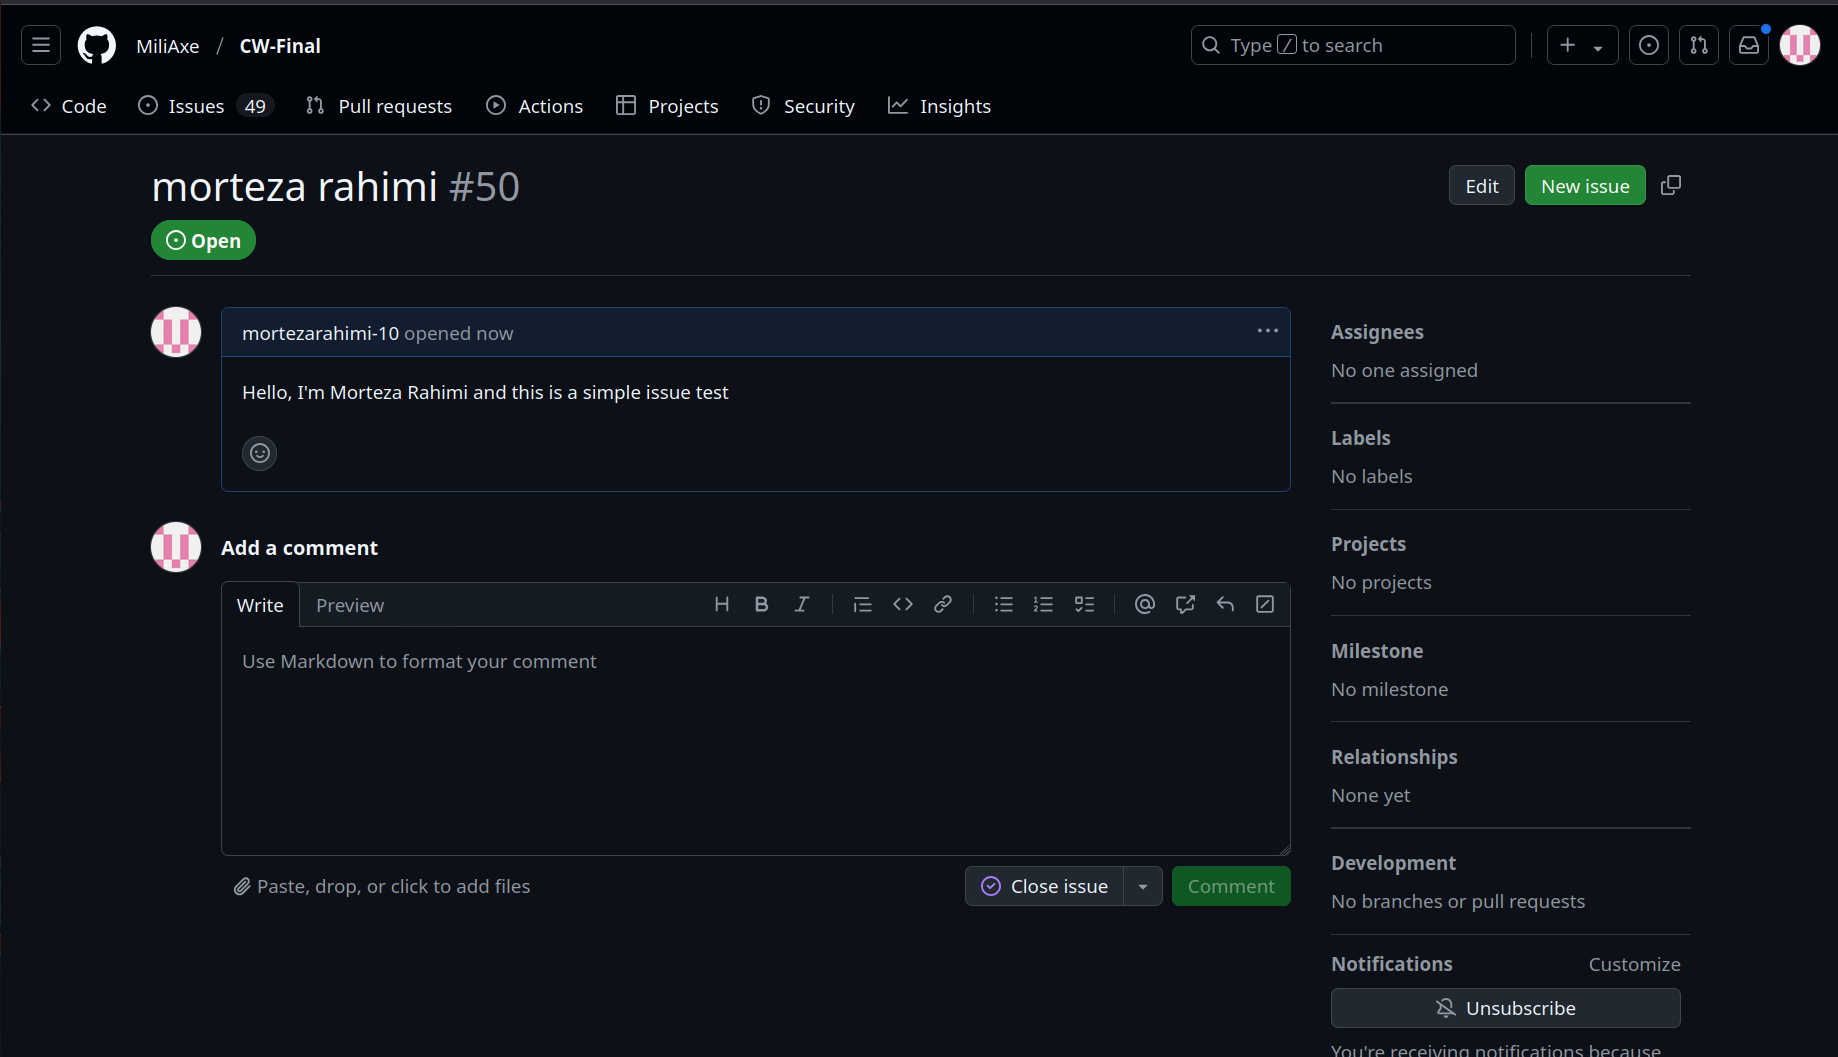
\includegraphics[width=0.8\textwidth]{./issue.jpg}
    \caption{this is the issue that i've created}
\end{figure}
\newpag
\subsection{FOSS contribution}
I think by contributing we learn new thing, So i wanna contribute to FOSS project that can teach me new things for example i don't wanna be professional in blockchain but i'm going to contribute in that field in the future.
\end{document}
